%u

\documentclass[12pt]{article}

\title{Research paper}
\author{Wessel Stoop, s0808709}

\usepackage{covington}
\usepackage{graphicx}

\renewcommand{\familydefault}{\sfdefault}

\begin{document}
\maketitle

\section{Introduction}

When one of Starfleet's vessels meets an alien ship in areas where no man has gone before, they can (almost) always communicate with these aliens (almost) instantly; they speak to them in English, and these aliens answer in English. This is possible because, according to the Star Trek lore, the protagonists make use of a so-called Universal Translator. This Universal Translator can (1) recognize speech in every language, (2) translate what it has 'heard' to any other language, (3) make its results audible with speech synthesis and (4) learn itself new languages when needed. Unfortunately, like many technologies in Star Trek, this is far from reality: there is lots of active research at the first three tasks in particular, but no software currently in existence can do this as perfect as the Universal Translator. \\\indent
In this paper, I will give a detailed overview of the research project Colibri, which basically is an attempt to improve the technology needed for the second task: automatically translating text from one language to another. More specifically, the project investigates the identification and extraction of constructions in natural language, and how these can be used in Machine Translation. These constructions can be of various lengths, and, importantly, can also contain one or more gaps. The constructions are not identified on the basis of explicit 'human' knowledge about language and grammar ('linguistic theory'), but are distilled from large amounts of text ('text corpora') with the help of context-sensitive machine-learning techniques. The Colibri project is carried out by Maarten van Gompel and supervised by Antal van den Bosch.







\section{Project description}

Besides an attempt to discover more about the possibilities for machine translation technology, Colibri is also an attempt to actually develop this technology. The following project overview therefore necessarily also is an overview of the software.

\subsection{Pattern extraction}

Colibri, 'Constructions as Linguistics Bridges', investigates constructions (or patterns), as its name suggests. A construction can be any group of consecutive words (a so-called 'n-gram') in any natural language that in some way forms an entity. An example is 'on the basis of' in the following sentence:

\begin{examples}
\item On the basis of these ideas, software can be developed.
\end{examples}

Importantly, constructions can also have one or more gaps (so-called 'skip-grams'). 'from \_\_ point of view' in the following example, is a construction with one such gap. 

\begin{examples}
\item I understand things better when I look at them from his point of view.
\end{examples}

The gap is filled here is filled with 'his', but the construction 'from \_\_ point of view' can also be filled with many other words ('my', 'the', 'another', 'Obama's', etc.). This shows the advantage of skip-grams over n-grams for machine translation: whereas n-grams would only have been able to capture the construction 'point of view', because the word directly before 'point of view' is variable, skip-grams are also able to recognize that the word 'for' is part of the construction.\\\indent
Of course, not every possible group of consecutive words is a construction; what makes some groups special? The exact nature of linguistic constructions has been the subject of many publications and even an entire linguistic framework (construction grammar). For this project however, it suffices to say that constructions emerge because some combinations of words are more frequent than others.

% Drie vormen freq: raw frequency, context frequency, multilingual alignmetn
% Blabla, want freq is waar mach learning gebriuk van maakt

\subsection{Pattern querying} Interactively query generated models for specific patterns.
\subsection{Pattern/corpus comparison} Match patterns generated from one corpus to another corpus.
\subsection{Graph computation \& visualisation} Compute graph relations between pattern models and visualise graphs
\subsection{Alignment algorithms} Algorithms to extract and align patterns accross languages; resulting in translation pairs for constructions.
\subsection{Machine Translation Decoding} Reassembles translated fragments into one coherent sentence in the target-language; seeking the best (statistically most probably) solution in a vast search space of possible search hypotheses.
\subsection{Memory-based Machine Translation} Machine learning algorithms can be used to consider source-side context in translations. Classifiers can be built and directly used by the decoder.
\subsection{Experiment Framework} Colibri comes with an extensive experiment framework for conducting Machine Translation experiments.\

\subsection{Hypotheses} %Of moet dit bij main outstanding questions?

Constructions can be found efficiently in corpus data
Graph-based relations can be used to constrain to good constructions
Constructions can be aligned without resorting to word alignments as a basis
In MT, constructions (i.e. possibly with gaps) result in better translation than mere consecutive phrases







\section{Theoretical background and framework}

\subsection{Classical Machine Translation}

Classical Machine Translation is best characterized by the use of human created rules. That is, authors of translation algorithms tried to include their knowledge about the languages and translation. There have been four main approaches, summarized in the Vauquois triangle: \\

\begin{figure}[htb]
\centering
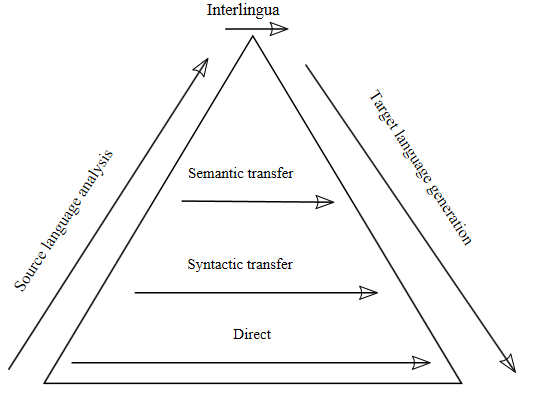
\includegraphics[width=0.8\textwidth]{vauquois.png}
\caption{The Vauquois triangle}
\label{fig:vauquois}
\end{figure}

The horizontal arrows represent the approaches, I'll go through them from bottom to top:

\begin{itemize}
\item The direct approach does very little source language analysis, and could thus be viewed as the automatical version of looking up every word in the source language in a dictionary and replacing it with the corresponding word in the target language. This often doesn't yield very good results: if I for example would have translated this paper from my mother tongue Dutch to English word for word, 'would we now not real a good result have'. It should be noted, however, that direct approach can be a little more intelligent than that: %wwat dan?
\item The syntactic approach
\item The semantic approach
\item All of the approaches so far have in common that they require a seperate rule set for each language pair; no or very few rules included for translations from English to German can also be used for translations from English to French. The Interlingua approach is an attempt to solve this problem, by pairing up every language with one general language, the Interlingua. This means a translation from English to German would entail a translation from English to the Interlingua (using the ruleset English $\rightarrow$ Interlingua) and then a translation from the Interlingua to German (using the ruleset Interlingua $\rightarrow$ German). When translating from English to French, the same two steps would be taken, and the same ruleset English $\rightarrow$ Interlingua can be used. This Interlingua is a formal representation.
\end{itemize}

% Voorbeelden?

\subsection{Statistical Machine Translation}












\section{Scientific importance and relevance for society}

% Ook lingusitic relevance: Abstracting fully lexicalised constructions
%Finding semantic subclasses in constructions: from time-expression to time-expression"
%Collapsing constructions with word disjunctions (\he/she/it") or part-of-speech tags
% Correlations with experimental findings
% Switch tasks, cloze tests, reaction times, ...

\section{Methodology}

% C++, Python

\section{Achievements so far}
\section{Main outstanding questions}
\section{Strengths and weaknesses}
\section{Possibilities for future research}
\section{Conclusion}

\section{References}

% Documentatie Colibri
% Maartens thesis

\end{document}
